\documentclass[runningheads]{llncs}

\usepackage[T1]{fontenc}

\usepackage{graphicx}

\begin{document}
	\title{Seminar- scientific methods in information systems}
	\subtitle{Predictive Process Monitoring Methods:\\ Which One Suits Me Best?}
	\author{Shuaiwei YU \inst{1} }
	\institute{Technical University of Munich\\
	\email{shuaiwei.yu@tum.de}}
	\maketitle
	
	%here begins the abstract
	\begin{abstract}
		The abstract should briefly summarize the contents of the paper in
		150--250 words.

		\keywords{First keyword  \and Second keyword \and Another keyword.}
	\end{abstract}
	
	%the first part: Introduction into the topic
	\section{Introduction}
	
	
	%the second part: Systematic Literature Review Protocol
	\section{Systematic Literature Review Protocol}
		%overview of the literature review.
		The research questions are formulated in the systematic literature review protocol, the search protocol is defined, and the selection criteria are developed. The selection criteria are based on the selection criterion of \cite{ref1} and are modified following the guideline provided in Kitchenham's article \cite{ref2}. The work consisted of several stages. In the first stage, The review protocol was designed. Specifically, the research questions to be investigated were formulated, and I chose the electronic database that will be used to run the search. The selection criteria, as well as inclusion criteria, were also defined. In the next stage, the horizontal search was run. The documents acquired were then filtered according to selection criteria; in the end, the final list of documents will be generated.
		
		%research questions development.
		The main research question (\textbf{RQ}):"\textit{What is the development and trend of the predictive process monitoring techniques over the research period?}" can be decomposed in four sub-question as follows. The first two sub-questions are so developed in order to research the current trends and algorithmic distribution of the predictive process monitoring. \textbf{RQ1}: "\textit{What is the distribution of the literature about predictive process monitoring over the search period?}" and \textbf{RQ2}: "\textit{What is the distribution of the algorithms used in predictive process monitoring over the search period?}". The next sub-question focuses on the aspects of outcome that can be predicted, \textbf{RQ3}:"\textit{What aspects can be predicted by the predictive process monitoring?}". In the last question, we want to research the reason that leads to the current trend of predictive process monitoring, i.e., \textbf{RQ4}: "What leads to the trend of predictive process monitoring?"
		
		%motivations of the research questions.
		In the first research question, we want to visualize the distribution of the article published in order to analyze the current trend of predictive process monitoring. With this visualization, we are able to take a deeper look into the development of interest in the industry of predictive process monitoring. The second research question examines the distribution of algorithms used for predictive process monitoring. The motivation for this is that we want to reveal which algorithms are more popular and widely used. With the first two research questions, we can derive the current research trend of predictive process monitoring. We can also analyze the possible research gaps where further academic contributions could be made. In \cite{ref1}, several aspects were already listed. However, the third research questions want to research whether there are new predictive aspects developed or how the new predictive process monitoring model predicts these aspects differently. The last research question tries to look into the reason that led to the current development of predictive process monitoring so that we might predict what the research direction of this field might be.
		
		%development of search string
		The search string must be defined so that we can query documents in an electronic database. We followed the guidelines and suggestions given by \cite{ref2} and based on the work of \cite{ref1}, we first chose the keywords "predictive", "prediction", "business process", and "process mining". Out of these four keywords, a search string can be built: ("predictive" OR "prediction") + ("business process" OR "process mining"). Furthermore, in order to explore as many results as possible, we also decided to add the keyword "process monitoring" to acquire more specific documents, so another search string is: ("predictive" OR "prediction") + "process monitoring". 
		
		%electronic database
		After defining the search string, we could choose electronic databases for searching. We decided to use Google Scholar as electronic databases to be used, for its completeness and simple operability. The search period was between year 2018 and 2022. We identified 263 hits initially with our keywords; after the search, we exported the results for further filtering.
		
		%steps of filtering below
		The first step of the filtering is about identifying the duplicates. Since several Databases are used, and the keywords can potentially overlap, our goal is to identify the literature that appeared more than once and whose name and author are identical. Only one of the papers will be preserved for future processes. After the duplicates filtering was performed, there were in total of 153 papers identified. In the next step, we look into the title of the papers gathered. In this step, (i) the studies that are related to a different field will be removed (e.g., "A Chemical Monitoring and Prediction System in Semiconductor Manufacturing Process Using Bigdata and AI Techniques", or "Condition monitoring and prediction of solution quality during a copper electroplating process"); (ii) the documents which are not proper research papers should also be removed (e.g., "Integration of an Explainable Predictive Process Monitoring System into IBM Process Mining Suite (Extended Abstract)"). The number of papers was reduced to 114 after filtering.
		
		%The last steps of filtering
		Moreover, we only consider the papers published in conferences, journals, and workshops, because, in comparison to degree thesis, published articles are more professional and have a higher academic contribution. After this stage of filtering, 106 papers are left. In the next stage of filtering, we looked into the abstract of each paper in order to evaluate its relevance. We also leave out the position paper at this stage since we only intended to look into the algorithms being used. After this filtering, 78 papers remained. In the last stage, we use the inclusion criterion \textit{"the study should propose a novel algorithm or technique for predictive process monitoring"} to further select the papers used for our study. We selected 28 papers in total, and through a backward reference search, 4 papers were added.
		
		\begin{figure}
		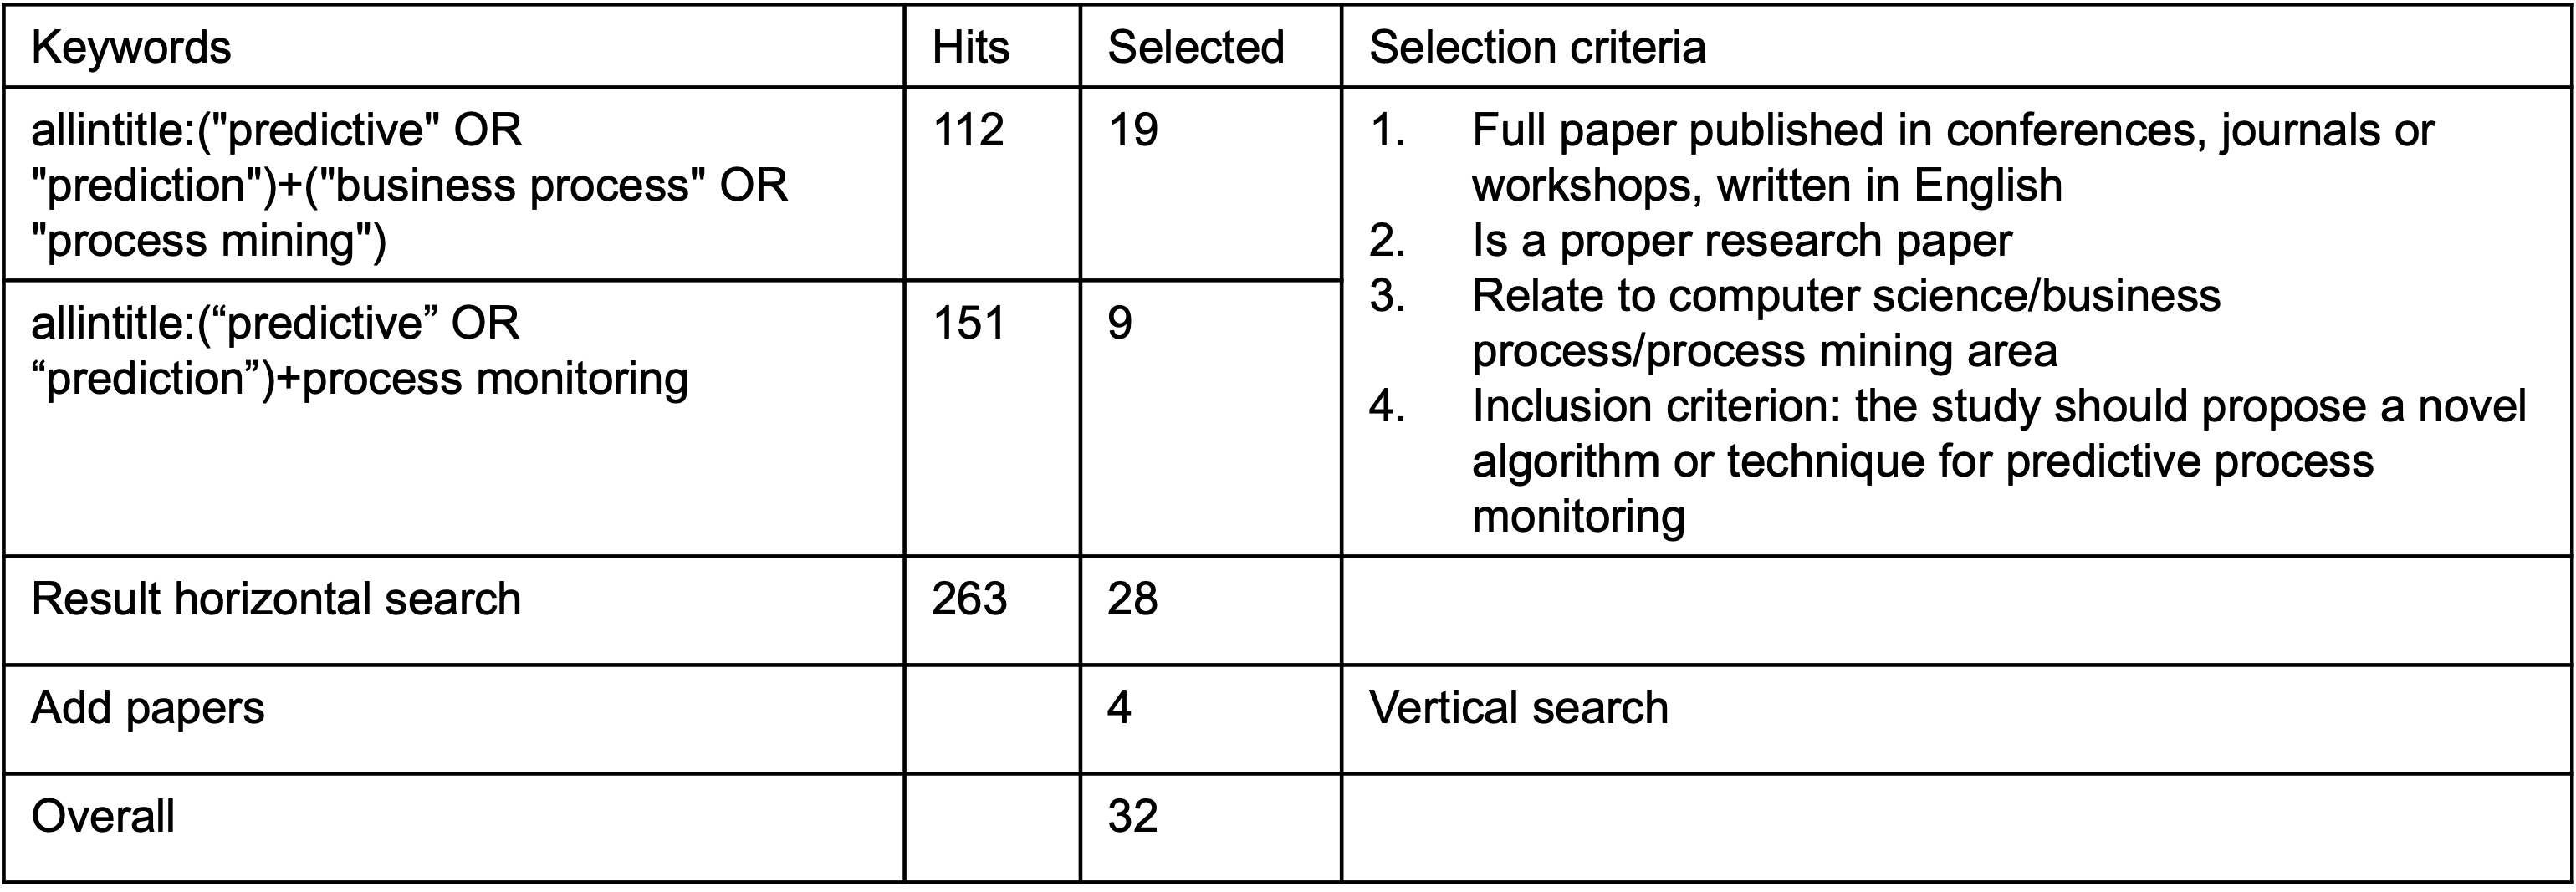
\includegraphics[width=\textwidth]{Filtering.png}
		\caption{Overview of Systematic Literature Review Protocol} \label{fig1}
		\end{figure}
		

		
	\section{Systematic Literature Review Results}





		
	\newpage
	\begin{thebibliography}{99}
	
	%TODO: 引用的格式???
	\bibitem{ref1}
	Di Francescomarino C, Ghidini C, Maggi F M, et al. Predictive process monitoring methods: Which one suits me best?[C]//International conference on business process management. Springer, Cham, 2018: 462-479.
	
	\bibitem{ref2}
	Kitchenham B. Procedures for performing systematic reviews[J]. Keele, UK, Keele University, 2004, 33(2004): 1-26.
		
	\end{thebibliography}

	
\end{document}
